%    This file is part of amc2moodle, a convertion tool to recast quiz written
%    with the LaTeX format used by automuliplechoice 1.0.3 into the 
%    moodle XML quiz format.
%    Copyright (C) 2016  Benoit Nennig, benoit.nennig@supmeca.fr 
%
%    This program is free software: you can redistribute it and/or modify
%    it under the terms of the GNU General Public License as published by
%    the Free Software Foundation, either version 3 of the License, or
%    (at your option) any later version.
%
%    This program is distributed in the hope that it will be useful,
%    but WITHOUT ANY WARRANTY; without even the implied warranty of
%    MERCHANTABILITY or FITNESS FOR A PARTICULAR PURPOSE.  See the
%    GNU General Public License for more details.
%
%    You should have received a copy of the GNU General Public License
%    along with this program.  If not, see <http://www.gnu.org/licenses/>.

\documentclass[a4paper]{article}

%#########################################################################
\usepackage{verbatim}
\usepackage[utf8]{inputenc}
\usepackage[T1]{fontenc}
%\usepackage[francais]{babel}
\usepackage{lmodern}
%\usepackage[hmargin=3cm, vmargin=1cm, includeheadfoot]{geometry}
\usepackage{amsmath,amssymb}
\usepackage{color}
\usepackage{graphicx}
\usepackage{subfigure}
\usepackage{framed}
\usepackage{hyperref}
\usepackage[final]{pdfpages} 
\hypersetup{pdfborder = 0 0 0}
\usepackage{breakurl}

%#########################################################################
\title{\texttt{amc2moodle}}

\author{B. Nennig\footnote{\url{benoit.nennig@supmeca.fr}}}

\newcommand{\elem}[1]{\texttt{<#1>}}
\newcommand{\py}{\texttt{grading.py}~}
\newcommand{\amc}{\texttt{amc2moodle}}


\begin{document}
%#########################################################################
%===================================================================
\maketitle 

%===================================================================
\begin{abstract}
	\input{../README.md}
\end{abstract}


% ========================================================================
\tableofcontents	
% ========================================================================
\newpage
\section{Install}
% ========================================================================
Dependencies :
\begin{itemize}
	\item install python [tested with 2.7] and lxml library (ubuntu using python package manager pip: sudo pip install lxml)
    \item install \texttt{PythonMagick} [tested with version 0.9.7-2] (ubuntu : sudo apt-get install python-pythonmagick). Useful to convert image files (*.eps, *.pdf, ...) into png.
    \item install \texttt{LateXML}\footnote{\url{http://dlmf.nist.gov/LaTeXML}} [tested with version 0.8.1] from package (ubuntu : sudo apt-get install latexml) or from source. If you choose to compile it, please check on :   
     \url{http://dlmf.nist.gov/LaTeXML/get.html}  that all the dependencies are installed. This program does the first step of the conversion into XML. Note that some version of \texttt{latexml} present an error in  
\begin{verbatim}
   /usr/share/perl5/LaTeXML/Common/Error.pm line 364.  
   To fix it, change line 364 in Error.pm to [[:cntrl:]]
   see https://bugs.debian.org/cgi-bin/bugreport.cgi?bug=839639
     \end{verbatim}
    \item install \texttt{xmlindent} [optional]. This program can be used to indent well the XML file (ubuntu : sudo apt-get install xmlindent). If not present just comment the call in the end of \texttt{amc2moodle.sh}.
\end{itemize}



Install :
\begin{itemize}
     \item Create a link in /usr/bin or add to the execution \amc~ root path the folder.
     \item Set the \texttt{src} folder in the \texttt{amc2moodle.sh} script or modify it to take into account an environment variable.
\end{itemize} 


Note : The project \texttt{TeX2Quiz}, \url{https://github.com/hig3/tex2quiz}, is a similar project to translate multiple choice quiz into moodle XML, without connexion with AMC.


\section{Usage}
% ========================================================================
\subsection{Command line call}
%-----------------------------------------------------------------------
Here is recall the \amc~-h output. Note that, ``\textbackslash'', stands for a line break.
%\begin{verbatim}
\verbatiminput{usage.txt}
%\end{verbatim}



\subsection{Code structure}
%-----------------------------------------------------------------------
The command line calls a shell script \texttt{amc2moodle.sh}. This script then call
\begin{itemize}
\item \texttt{LateXML} with \texttt{automuliplechoice.sty.ltxml}. The package has been made using \texttt{note} element in LateXML and most of  AMC environment or command names are pass through attribute (in french for the moment). User command can be added in the .tex file. This first step is used to get an XML file \texttt{tex2xml.xml}. Thanks to \texttt{LateXML}, most \LaTeX possibilities are supported in the conversion to moodle. Note that option passed to \texttt{automuliplechoice.sty} package are ignored.

\item \py with \texttt{lxml} is used to add data like grade, image conversion and additional attributes to ease XSLT stylesheet transformation. For the moment, 3 layers of XSLT are use i) \texttt{transform\_ns.xslt} to remove the namespace added by \texttt{LateXML}, ii) \texttt{transform2html.xslt} to recast the image element, convert into html text style, tables and extract raw tex equations (instead of mathml). The html are embedded into CDATA markup.
Note that image elements will appear twice i) in \elem{img} elements present in the CDATA markup to html moodle rendering and ii) in \elem{file} element in order to embedded the image file as text (base64). This elements are present at \elem{questiontext} level or answer \elem{answer} level.
The last XSLT transform, performed by \texttt{transform.xslt} is used change the element name and conform to moodle XML format.
\end{itemize}
Note that i) moodle fill the missing element like feedback (see \ref{sec:feed}); ii) the global structure have been obtained by looking few questions created directly in moodle. 
% 

\subsection{What you can do}
% ========================================================================
\begin{itemize}
\item Convert \texttt{question} and \texttt{questionmult} environments.
\item You don't need to remove questionnaires part \textbackslash \texttt{exemplaire} or \textbackslash \texttt{onecopy}. But if this part contains undefined commands, remove/comment it!
\item Put in-line equations like $x^2$ or use equation environment (or \$\$ delimiters). For the moment eqnarray  or the amsmath environments multline, align are not supported. The choice have been made to keep equation in tex and use mathjax filter of moodle for rendering. In my opinion, it is better for modifying question after importation.
\item Include image, in all format supported by \texttt{PythonMagick}. \amc   will convert it in .png for moodle export. The image will be embedded as text (base64) in the output xml file. The folder is '/' in moodle. The image can be in an another folder than the tex file.
\item Include Table, with the tabular environment. In the present form, \amc put  border around each cell.
\item Use italic, typerwritter, bold, emphasize\dots
\item Automatically add an answer like ``there is no good answer'' if there is no good answer.
\item Use user's command defined in the \LaTeX~file.
\item \texttt{\textbackslash usepackage[utf8]\{inputenc\}}   for accents
\item Use packages that are supported by \texttt{LateXML}. See the list at \url{http://dlmf.nist.gov/LaTeXML/manual/included.bindings/}. Instead you need to add a binding to \texttt{LateXML}.
\end{itemize}

\subsection{What you cannot do}\label{sec:cannot}
% ========================================================================
\begin{itemize}
\item Use underscore in question name field !
\item Use verbatim. This environment is not supported by \texttt{automultiplechoice} 1.0.3. Use \texttt{alltt} package instead.
\item Use font size (easy to add)
\item Use amsmath environments like align, aligned\dots Because  \texttt{tex} attribute of \elem{equation}, provided by \texttt{LateXML} output, doesn't contains really the raw tex equation.
\item Change border of table
\item Use command like \texttt{\textbackslash raggedright}, text align is not fully supported. this add align information into the \texttt{class} attribute of \elem{note} and the string matching break down. Note that \texttt{\textbackslash raggedright} is bypassed. %in\texttt{/src/automultiplechoice.sty.ltxml}
\item Use \texttt{multicol}, it use is bypass \texttt{automultiplechoice.sty.ltxml} for choices layout. But it should be possible to use it elsewhere (create newcommand).
\item Translate equation into mathml, but it can be easily changed
\item Use AMC numeric question
\item Only the main commands of the package \texttt{automultiplechoice.sty} are supported in french. The english keywords support is on-going. The list of supported keywords can be seen in \texttt{/src/automultiplechoice.sty.ltxml}
\item You cannot remove the add of "None of these answers are correct" choice at the end of each multiple question.


\end{itemize}
 
\section{Grading strategy}
% ========================================================================
In moodle 3, %if the total grade is negative then the total grade for this question will be zero. 
the grading strategy is different from AMC especially for question with multiple answers. In this case, AMC affects a grade for each checked good answer and each non-checked wrong answer. The total grade of the question depend on the number of choice.

In Moodle and here, only checked item leads to a grade, positive or negative. The grading is compute in the \py script.
The defaut grading parameter are set in \py script to
\begin{verbatim}
# Multiple :: e :incohérence, b: bonne,  m: mauvaise,  p: planché
amc_bs = {'e':-1,'b':1,'m':-0.5}              
amc_bm = {'e':-1,'b':1,'m':-0.5, 'p':-1}   
# defaut question grade in moodle
moo_defautgrade = 1.                       
\end{verbatim}
This value can be changed (as in AMC) with the tex command
\begin{verbatim}
\baremeDefautS{e=-0.5,b=1,m=-0.5}         % never put b<1,
\baremeDefautM{e=-0.5,b=1,m=-0.25,p=-0.5} % never put b<1,
\end{verbatim}
or at the question level with the tex command \texttt{bareme}.
The gade $g_i$ in \% is then computed as
$g_i = 100\cdot c_i / N_i$ where $i$ stand for the good or the wrong answer. Here, $N_i$ is the total number of the good or the wrong answer and $c_i$ the coefficient (\texttt{m}, \texttt{b}\dots). It important to set b=1 to get 100\% if all the good answers are found. The \texttt{e} parameter is not used here, because it is not possible to tick 2 answers in moodle for one-answer-question. The only case where incoherent can be used is if the ``\emph{there isn't any correct answer''} answer is ticked with another question but it is not implemented.

Another difference is that moodle 3 use tabulated grade like : 1/2, 1/3, 1/4, 1/5, 1/6, 1/7, 1/8, 1/9, 1/10 and their multiple. If your grade are not conform to that you must use : 'Nearest grade if not listed' in import option in the moodle question bank. But check at least that the sum of good answer give 100\% !




 
\section{Categories}
% ========================================================================
By default, the imported questions are all created in \texttt{$course$/filein}  . When the flag \texttt{-c} is used, the AMC command \texttt{element} is used to create subcategories and the argument following \texttt{-c catname} is used instead of \texttt{filein}.
Each question is then placed in \texttt{$course$/catname/elementName}.
This part is set in \py.

\section{Feedback}\label{sec:feed}
% ========================================================================
Feedback are present, in a certain way, in \texttt{automuliplechoice} with the \textbackslash\texttt{explain} command. This part is not yet implemented in \amc. However it could be easy to add it at the response or question level as other fields and bypass them for real \texttt{automuliplechoice} test.


\section{Import in Moodle}
% ========================================================================


\section{Example}
% ========================================================================
A complete example to illustrate the possibilities of \amc, is given in \texttt{/test/QCM.tex}, an extract is given below to illustrate the syntax 
\begin{verbatim}
\element{cat1}{    % use category and sub-category to classify questions
	\begin{questionmult}{QLabel}  
		\bareme{e=-0.5,b=1,m=-1.,p=-0.5} % never put b<1,
		Quel fruit possède un noyau ?
		  \begin{reponses}    
		    \mauvaise{La pomme}
		    \mauvaise{La tomate}
		    \mauvaise{le Kiwi}
		  \end{reponses}
	\end{questionmult}
}
\end{verbatim}
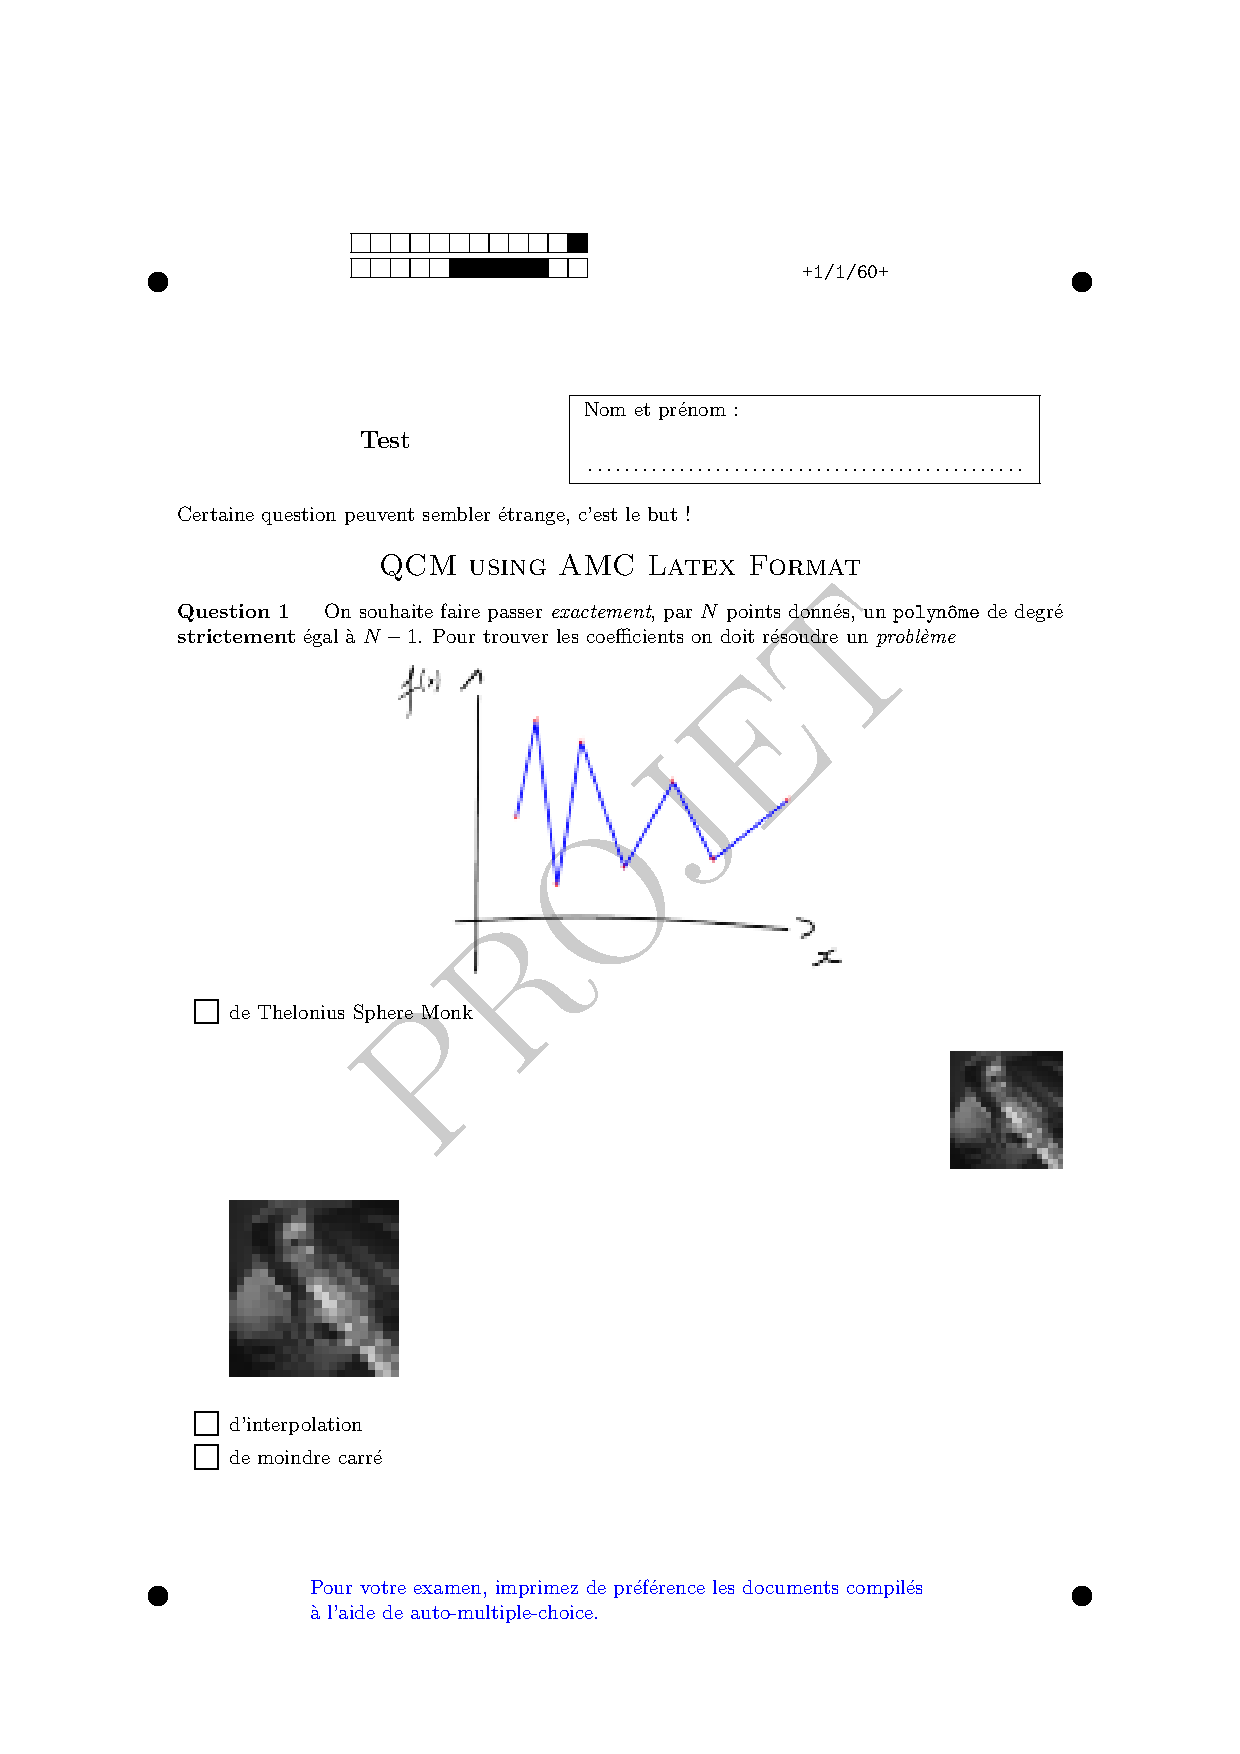
\includepdf[pages=-,scale=.95,nup=1x2,landscape,
pagecommand={\thispagestyle{plain}},linktodoc=false,
addtotoc={1,subsection,1,AMC example,sec:exQCM}]{../test/QCM.pdf}


\section{To do list}
% ========================================================================
All the points listed in sec.~\ref{sec:cannot} can be push on this list, among them
\begin{itemize}
\item Add mathml support
\item Add other equation environnement in raw tex
\item All multi-langage support of \texttt{automultiplechoice.sty} and really implement all the \texttt{automultiplechoice.sty} command!
\item Add AMC numeric question support
\item Add a support for listing or verbatim environment. For the moment, \texttt{alltt} seems to be supported.
\item Add a support for feedback with \textbackslash\texttt{explain} command
\end{itemize}
\end{document}
